\section{Empirical validation of our theoretical insights}
\label{sect:analysis}
We consider several collections of weights $\{\theta_{m}\}_{m=1}^M$ ($2\leq M < 10$) trained on the \enquote{Clipart}, \enquote{Product} and \enquote{Photo} domains from OfficeHome \cite{venkateswara2017deep} with a shared random initialization and mild hyperparameter ranges.
These weights are first indifferently sampled from a single run (every $50$ batches) or from different runs.
They are evaluated on \enquote{Art}, the fourth domain from OfficeHome.%
\begin{figure}
% \centering
\begin{minipage}{.45\textwidth}%
  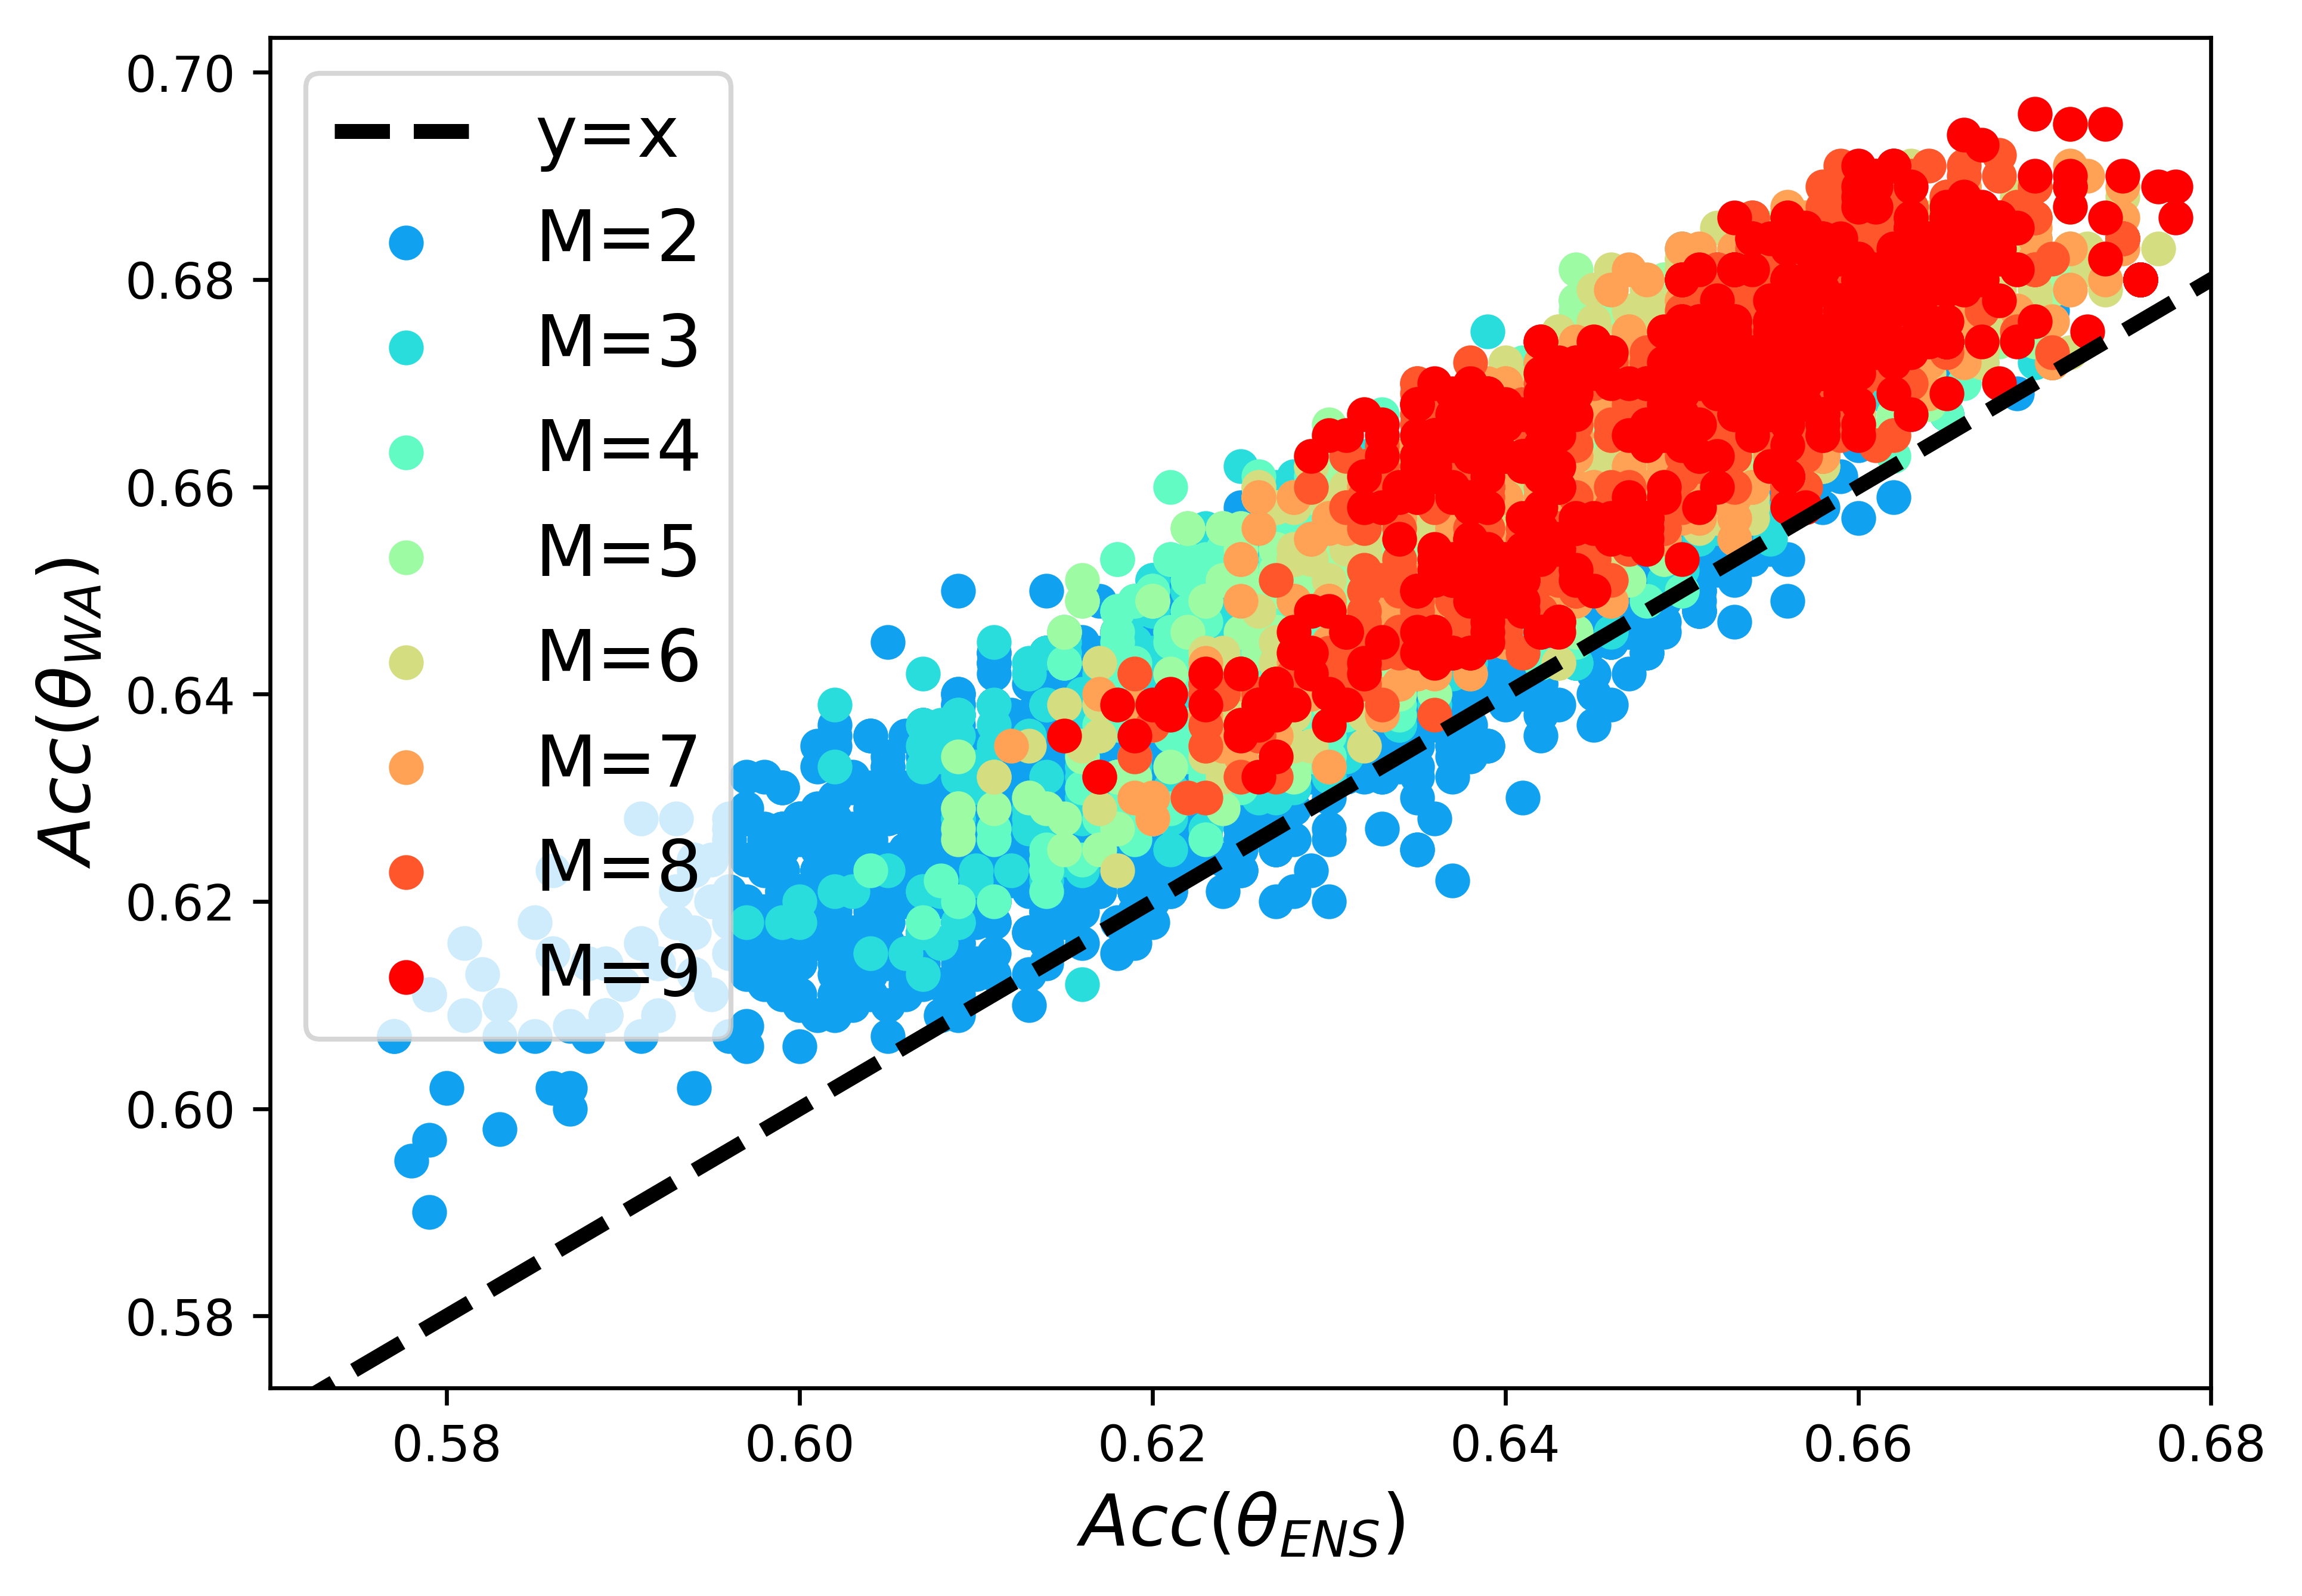
\includegraphics[width=\linewidth]{pictures/files/final/home0_samediffruns210_ens_wa_57.png}
%   \vspace{-0.2em}%
  \captionof{figure}{Each dot displays the accuracy ($\uparrow$) of weight averaging (WA) \versus accuracy ($\uparrow$) of prediction averaging (ENS) for $M$ models.}
  \label{fig:home0_samediffruns_net_soup}
\end{minipage}%
\hskip 4ex
\begin{minipage}{.45\textwidth}%
  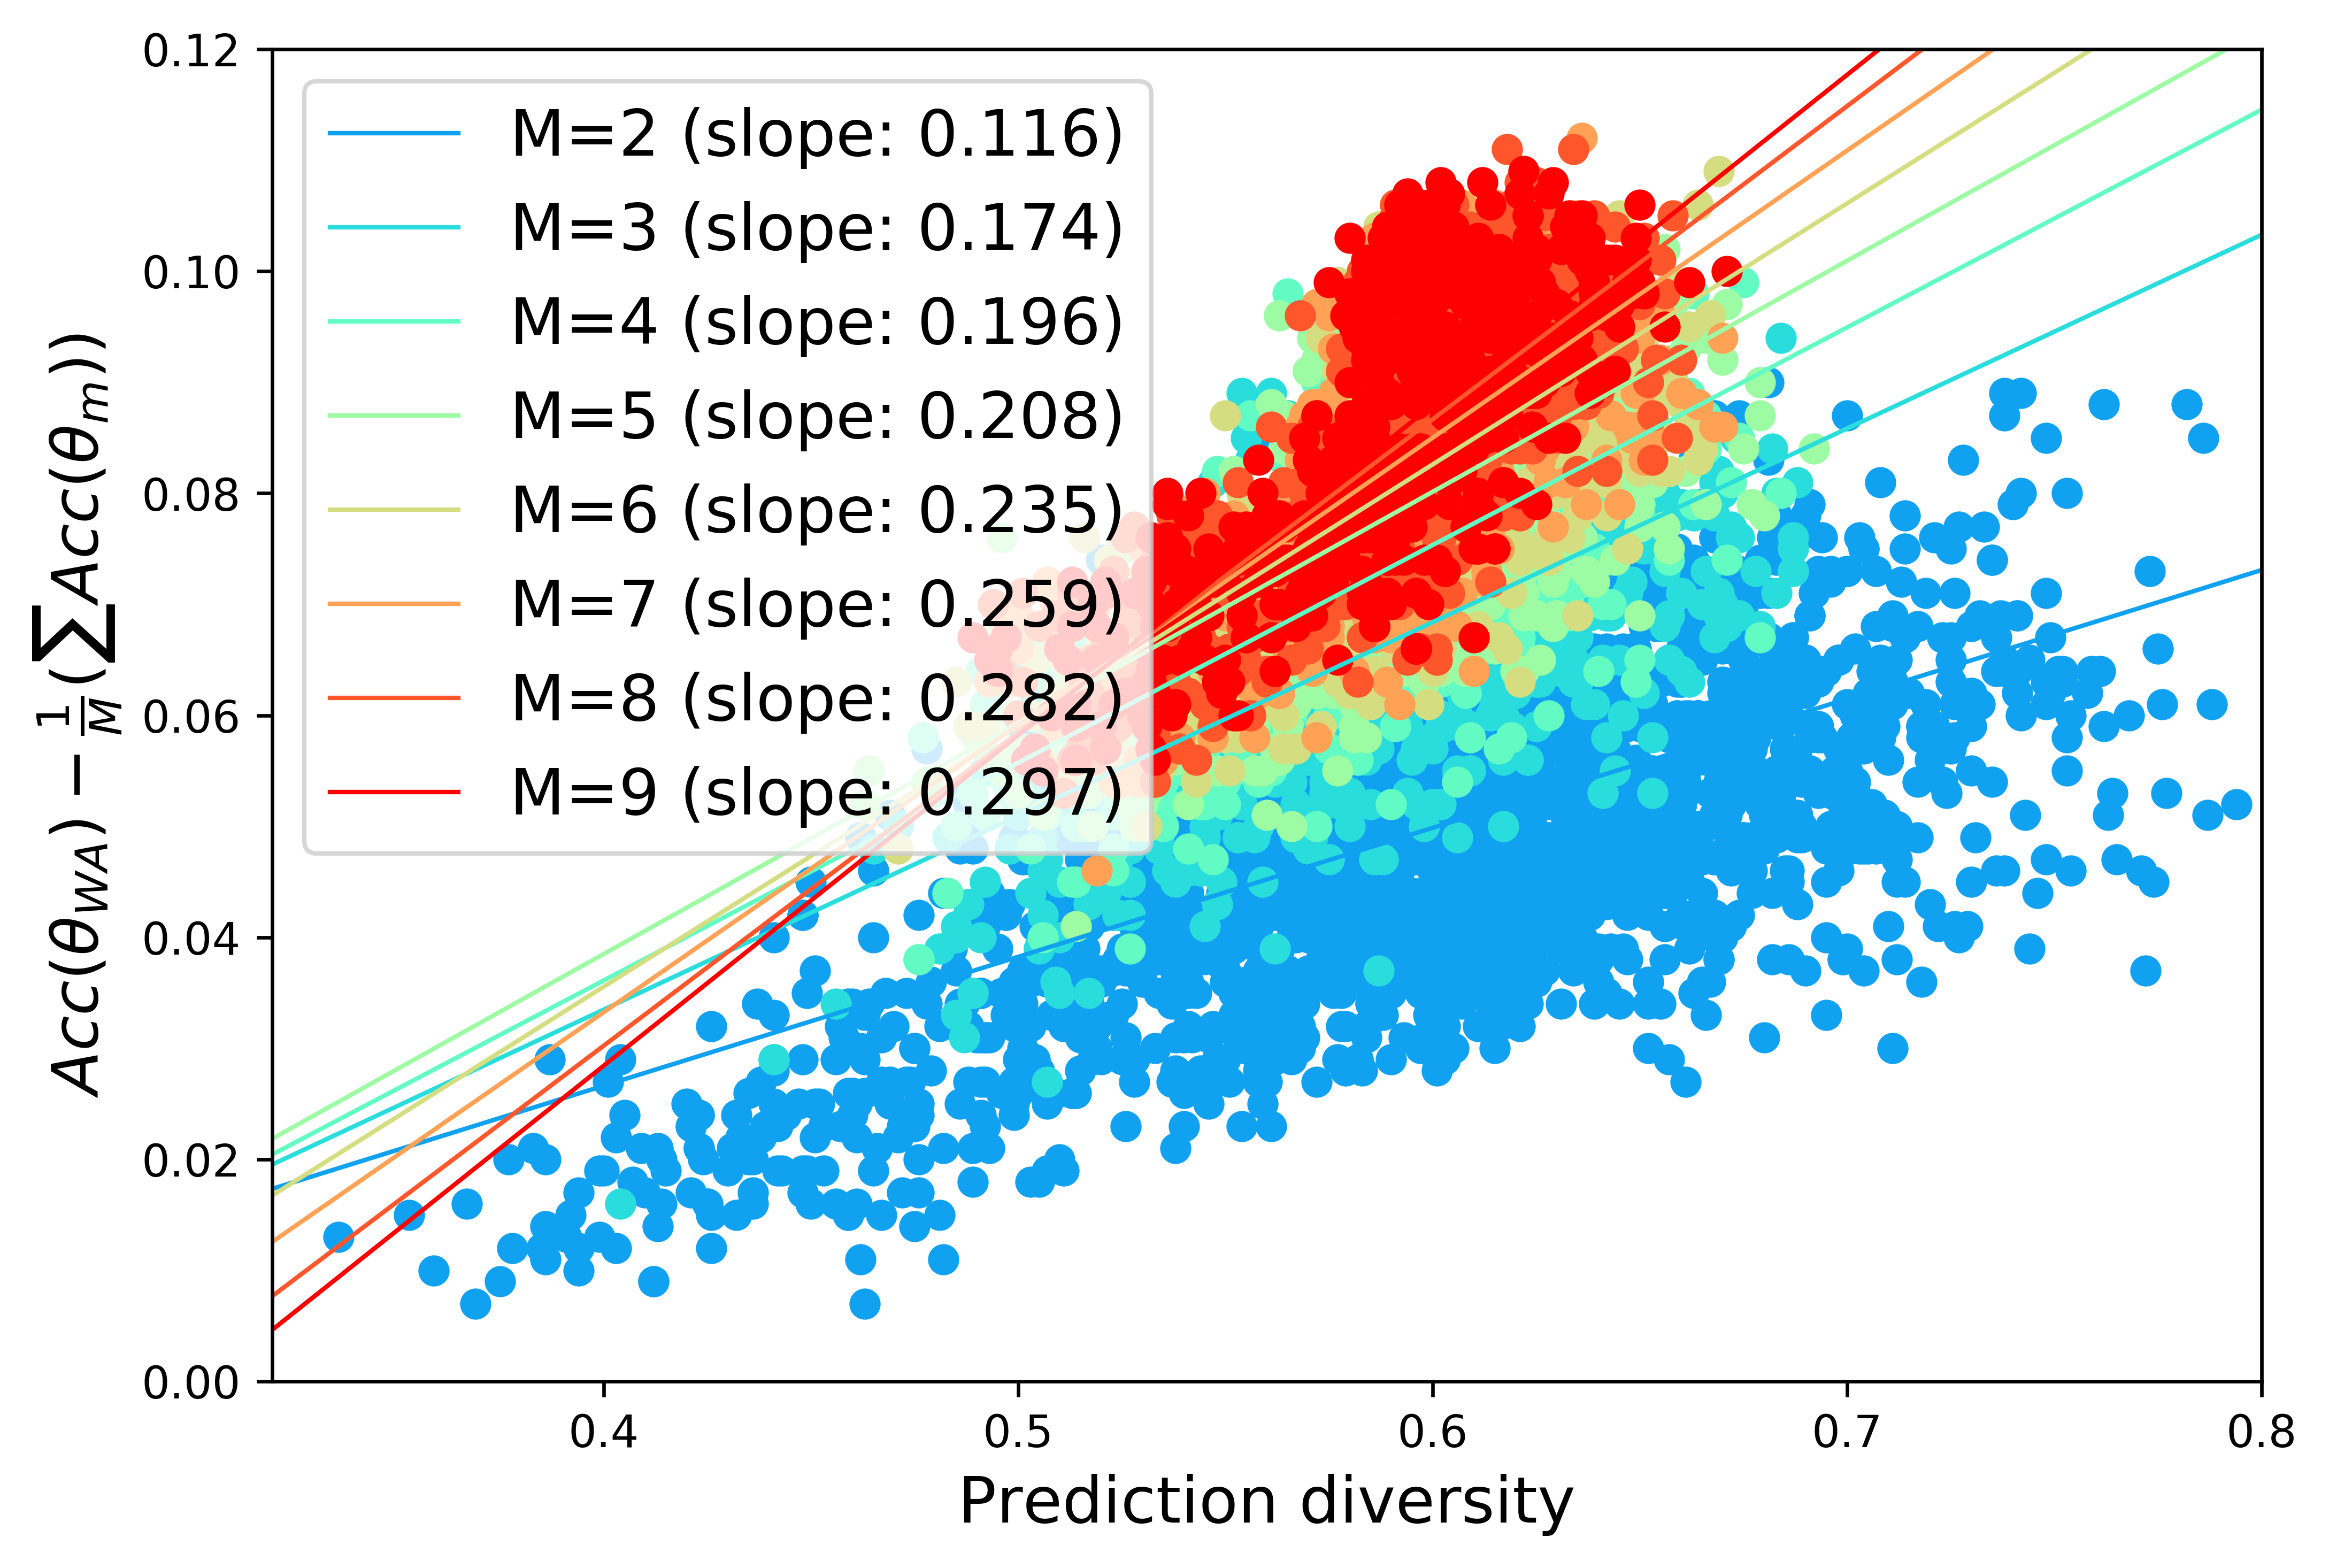
\includegraphics[width=\linewidth]{pictures/files/final/home0_samediffruns_dr_soup-netm.png}
  \captionof{figure}{Each dot displays the accuracy ($\uparrow$) gain of WA over its members \versus the prediction diversity \cite{aksela2003comparison} ($\uparrow$) for $M$ models.}
  \label{fig:home0_dr_soup-netm}
\end{minipage}
% \vspace{-1.em}%
\end{figure}

\paragraph{WA \versus ENS.}
\Cref{fig:home0_samediffruns_net_soup} validates \Cref{lemma:wa_ensembling} and that \textbf{$f_{\text{WA}} \approx f_{\text{ENS}}$}. 
More precisely, $f_{\text{WA}}$ slightly but consistently improves $f_{\text{ENS}}$: we discuss this in \Cref{app:wa_vs_ens_analysis}.
Moreover, a larger $M$ improves the results; in accordance with \Cref{eq:b_var_cov}, this motivates averaging as many weights as possible.
In contrast, large $M$ is computationally impractical for ENS at test time, requiring $M$ forwards.%

\paragraph{Diversity and accuracy.}
% \vspace{-1em}%
We validate in \Cref{fig:home0_dr_soup-netm} that $f_{\text{WA}}$ benefits from diversity.
Here, we measure diversity with the ratio-error \cite{aksela2003comparison}, \ie the ratio $N_{\text{diff}}/N_{\text{simul}}$ between the number of different errors $N_{\text{diff}}$ and of simultaneous errors $N_{\text{simul}}$ in test for a pair in $\{f\left(\cdot, \theta_{m}\right)\}_{m=1}^M$.
A higher average over the $\binom{M}{2}$ pairs means that members are less likely to err on the same inputs.
Specifically, the gain of $\operatorname{Acc}(\theta_{\text{WA}})$ over the mean individual accuracy $\frac{1}{M}\sum_{m=1}^M\operatorname{Acc}\left(\theta_m\right)$ increases with diversity.
Moreover, this phenomenon intensifies for larger $M$: the linear regression's slope (\ie the accuracy gain per unit of diversity) increases with $M$. This is consistent with the $(M-1)/M$ factor of $\covb\left(x\right)$ in \Cref{eq:b_var_cov}, as further highlighted in \Cref{app:soup:m_slope}.
Finally, in \Cref{app:analysis_office_features}, we show that the conclusion also holds with CKAC \cite{DBLP:journals/corr/abs-1905-00414}, another established diversity measure.

\paragraph{Increasing diversity thus accuracy via different runs.}
Now we investigate the difference between sampling the weights from a single run or from different runs.
\Cref{fig:home0_dr_frequency} \textit{first} shows that diversity increases when weights come from different runs.
\textit{Second}, in \Cref{fig:home0_m_vs_acc}, this is reflected on the accuracies in \ood.
Here, we rank by validation accuracy the $60$ weights obtained (1) from $60$ different runs and (2) along $1$ well-performing run.
We then consider the WA of the top $M$ weights as $M$ increases from $1$ to $60$.
Both have initially the same performance and improve with $M$; yet,
% because weights from different runs are more diverse, their WA performs better.
WA of weights from different runs gradually outperforms the single-run WA.
\textit{Finally}, \Cref{fig:home0_locality_requirement} shows that this holds only for mild hyperparameter ranges and with a shared initialization.
Otherwise, when hyperparameter distributions are extreme (as defined in \Cref{tab:hyperparam}) or when classifiers are not similarly initialized, DiWA may perform worse than its members due to a violation of the locality condition.
These experiments confirm that \textit{diversity is key as long as the weights remain averageable}.%
% \begin{figure}[h]%
%     % \vspace{-3em}%
%     \centering%
%     \begin{subfigure}{.33\textwidth}%
%         \centering%
%         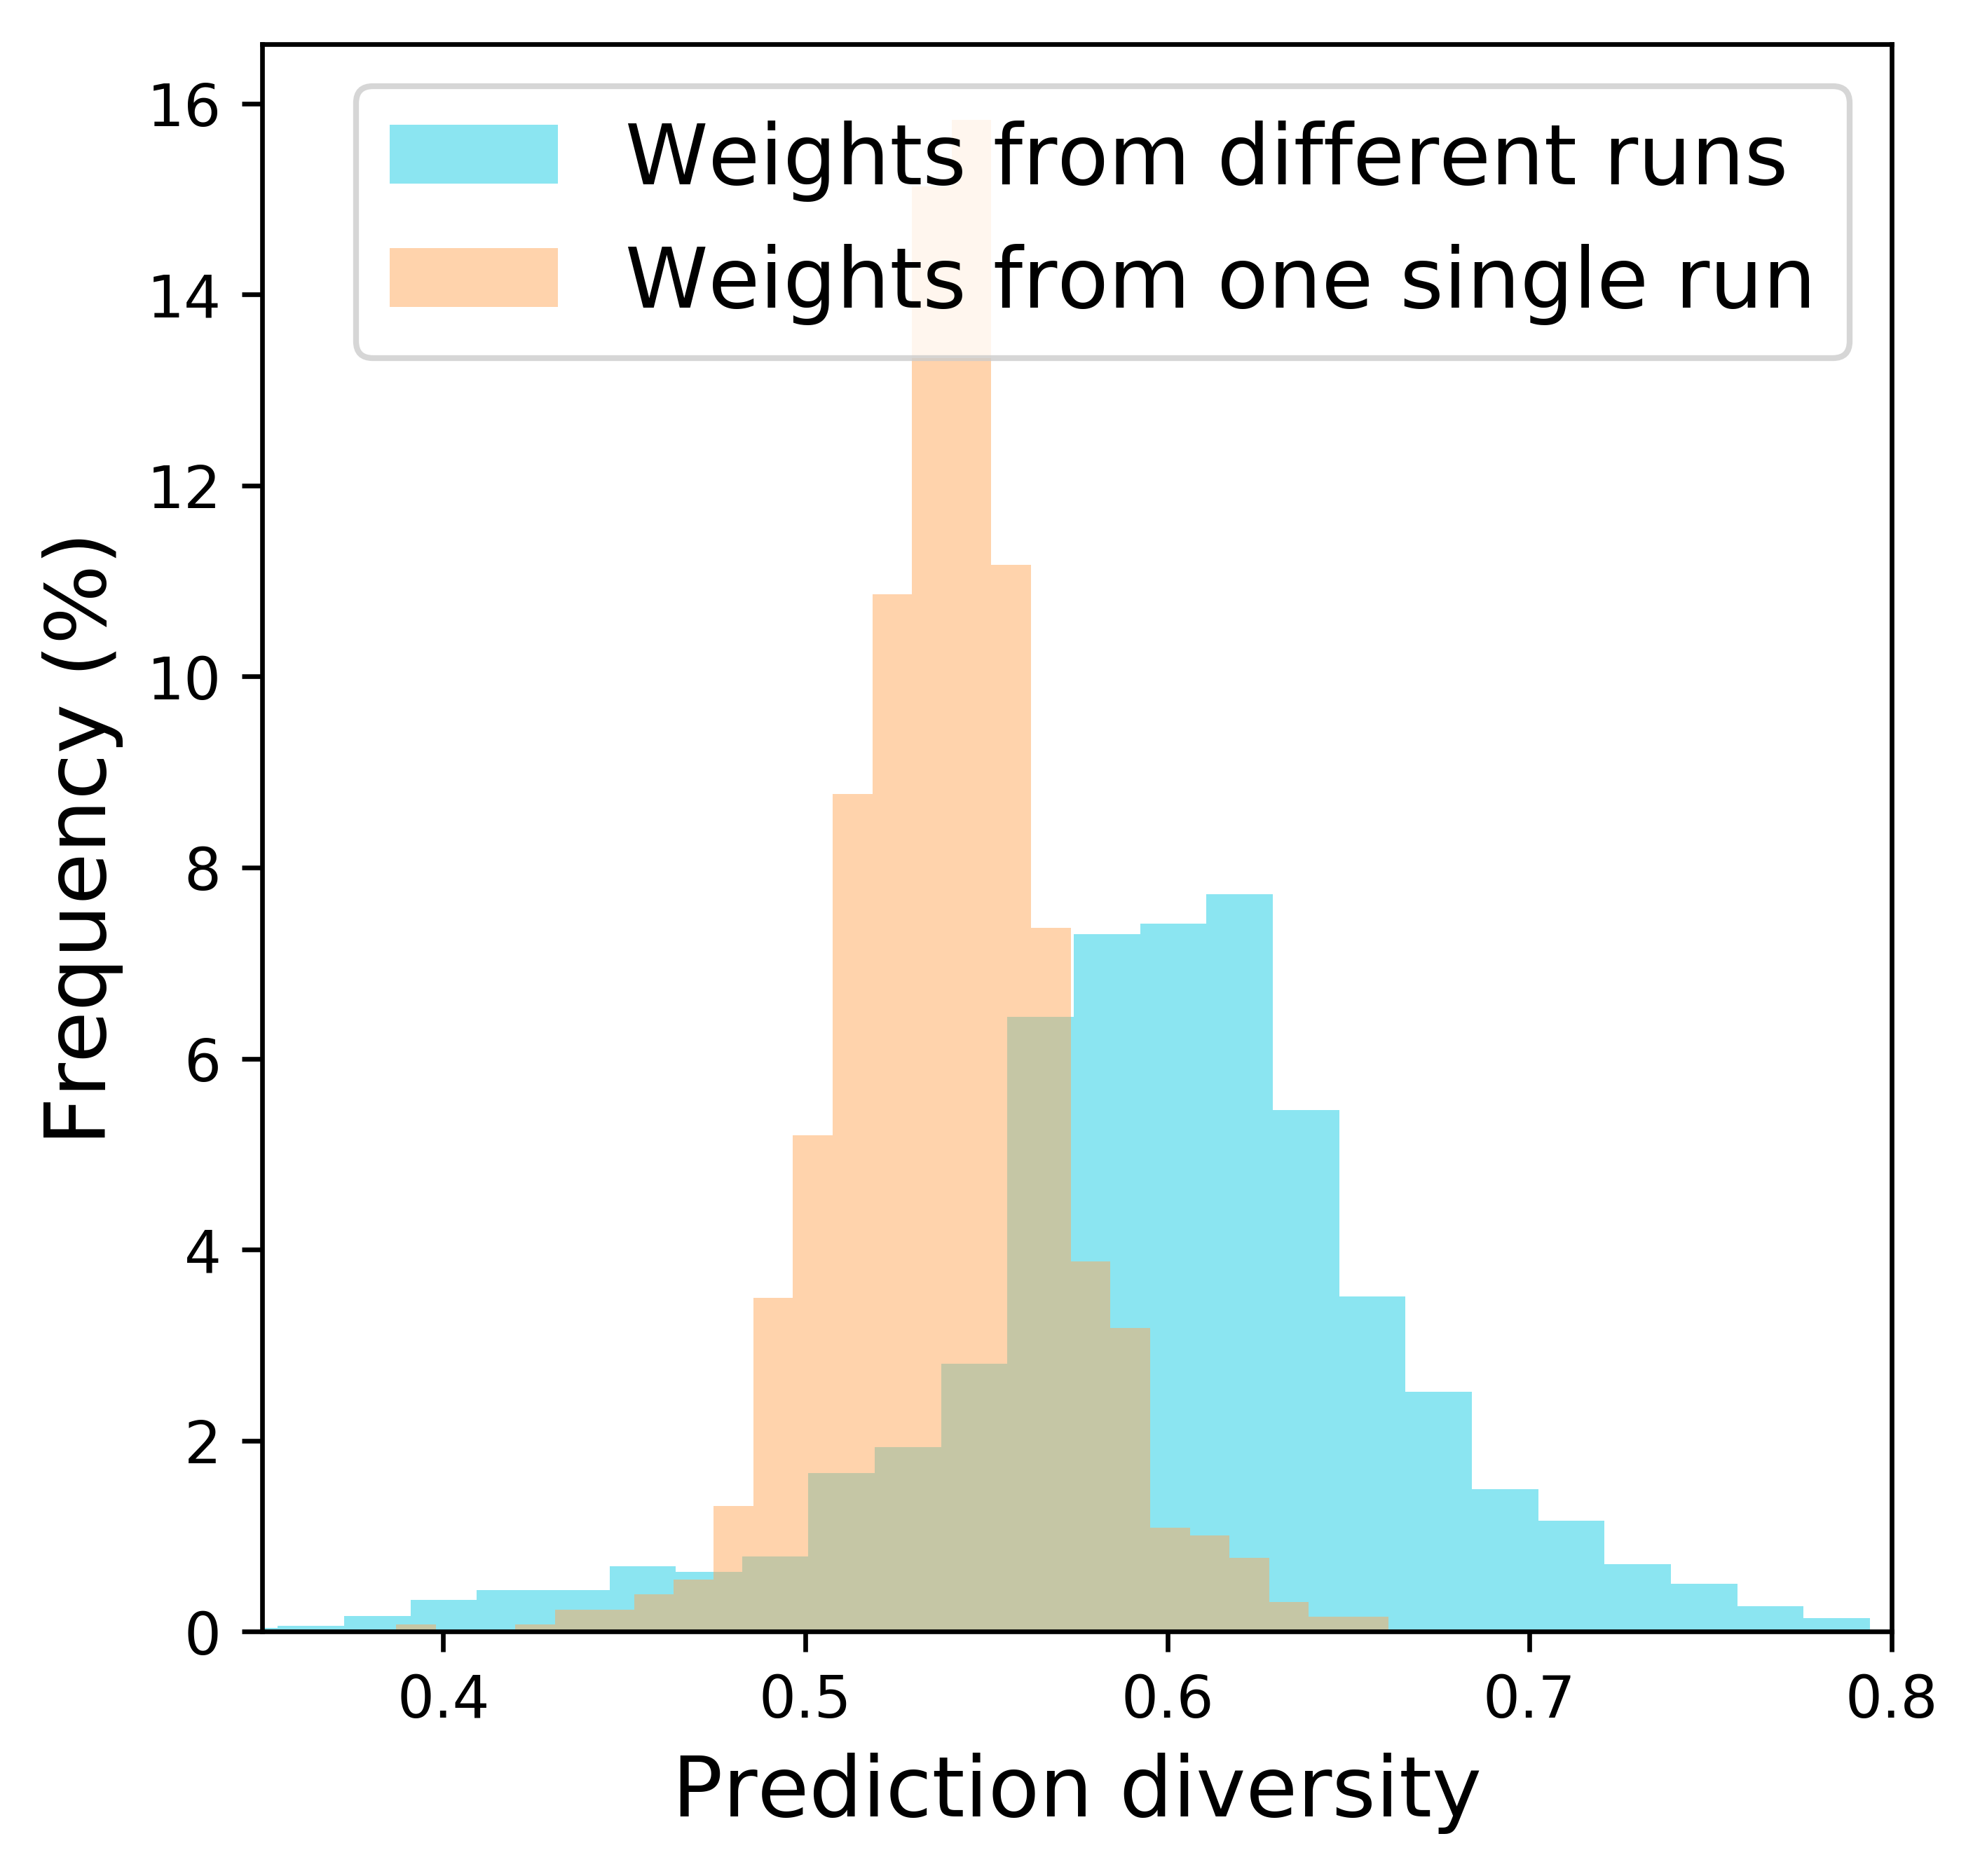
\includegraphics[width=0.9\textwidth]{pictures/files/final/home0_hist_dr.png}%
%         \caption{Diversity ($\uparrow$) across weights.}%
%         \label{fig:home0_dr_frequency}
%     \end{subfigure}%
%     \begin{subfigure}{.33\textwidth}%
%         \centering%
%         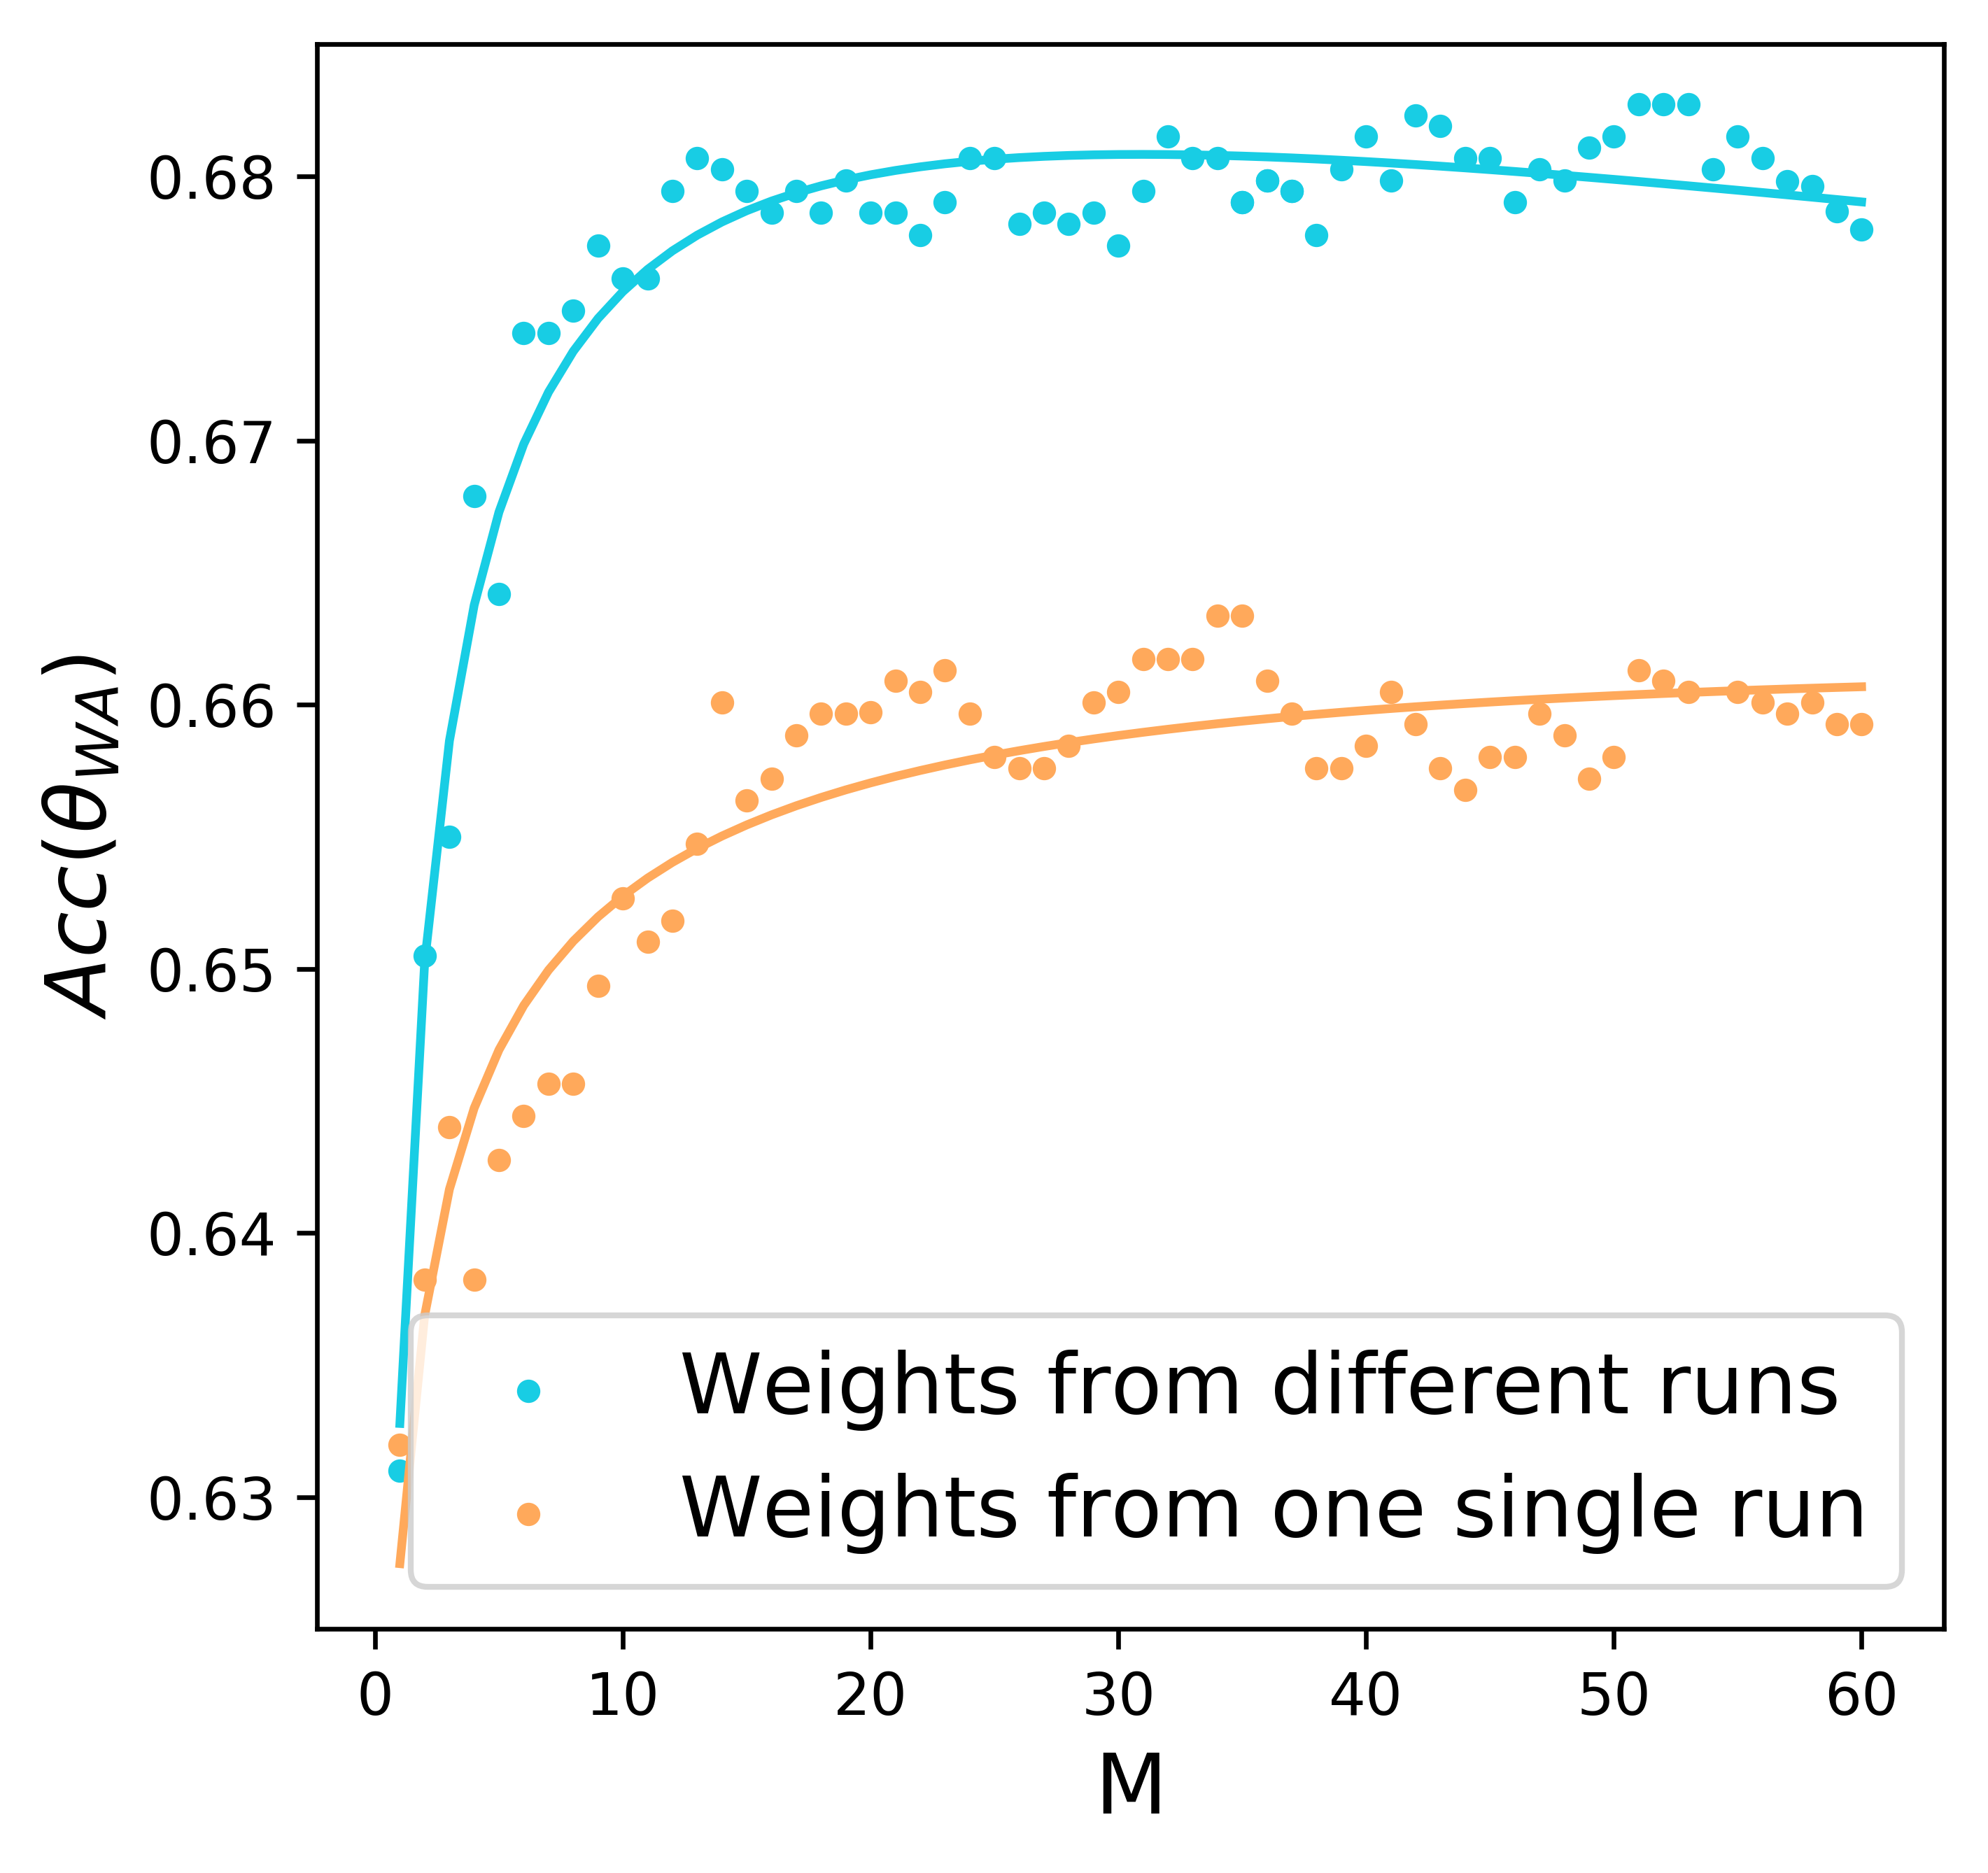
\includegraphics[width=0.9\textwidth]{pictures/files/final/home0_samediffruns_m_soup_ood.png}%
%         \caption{WA accuracy ($\uparrow$) as $M$ grows.}%
%         \label{fig:home0_m_vs_acc}%
%     \end{subfigure}%
%     \begin{subfigure}{.33\textwidth}%
%         \centering%
%         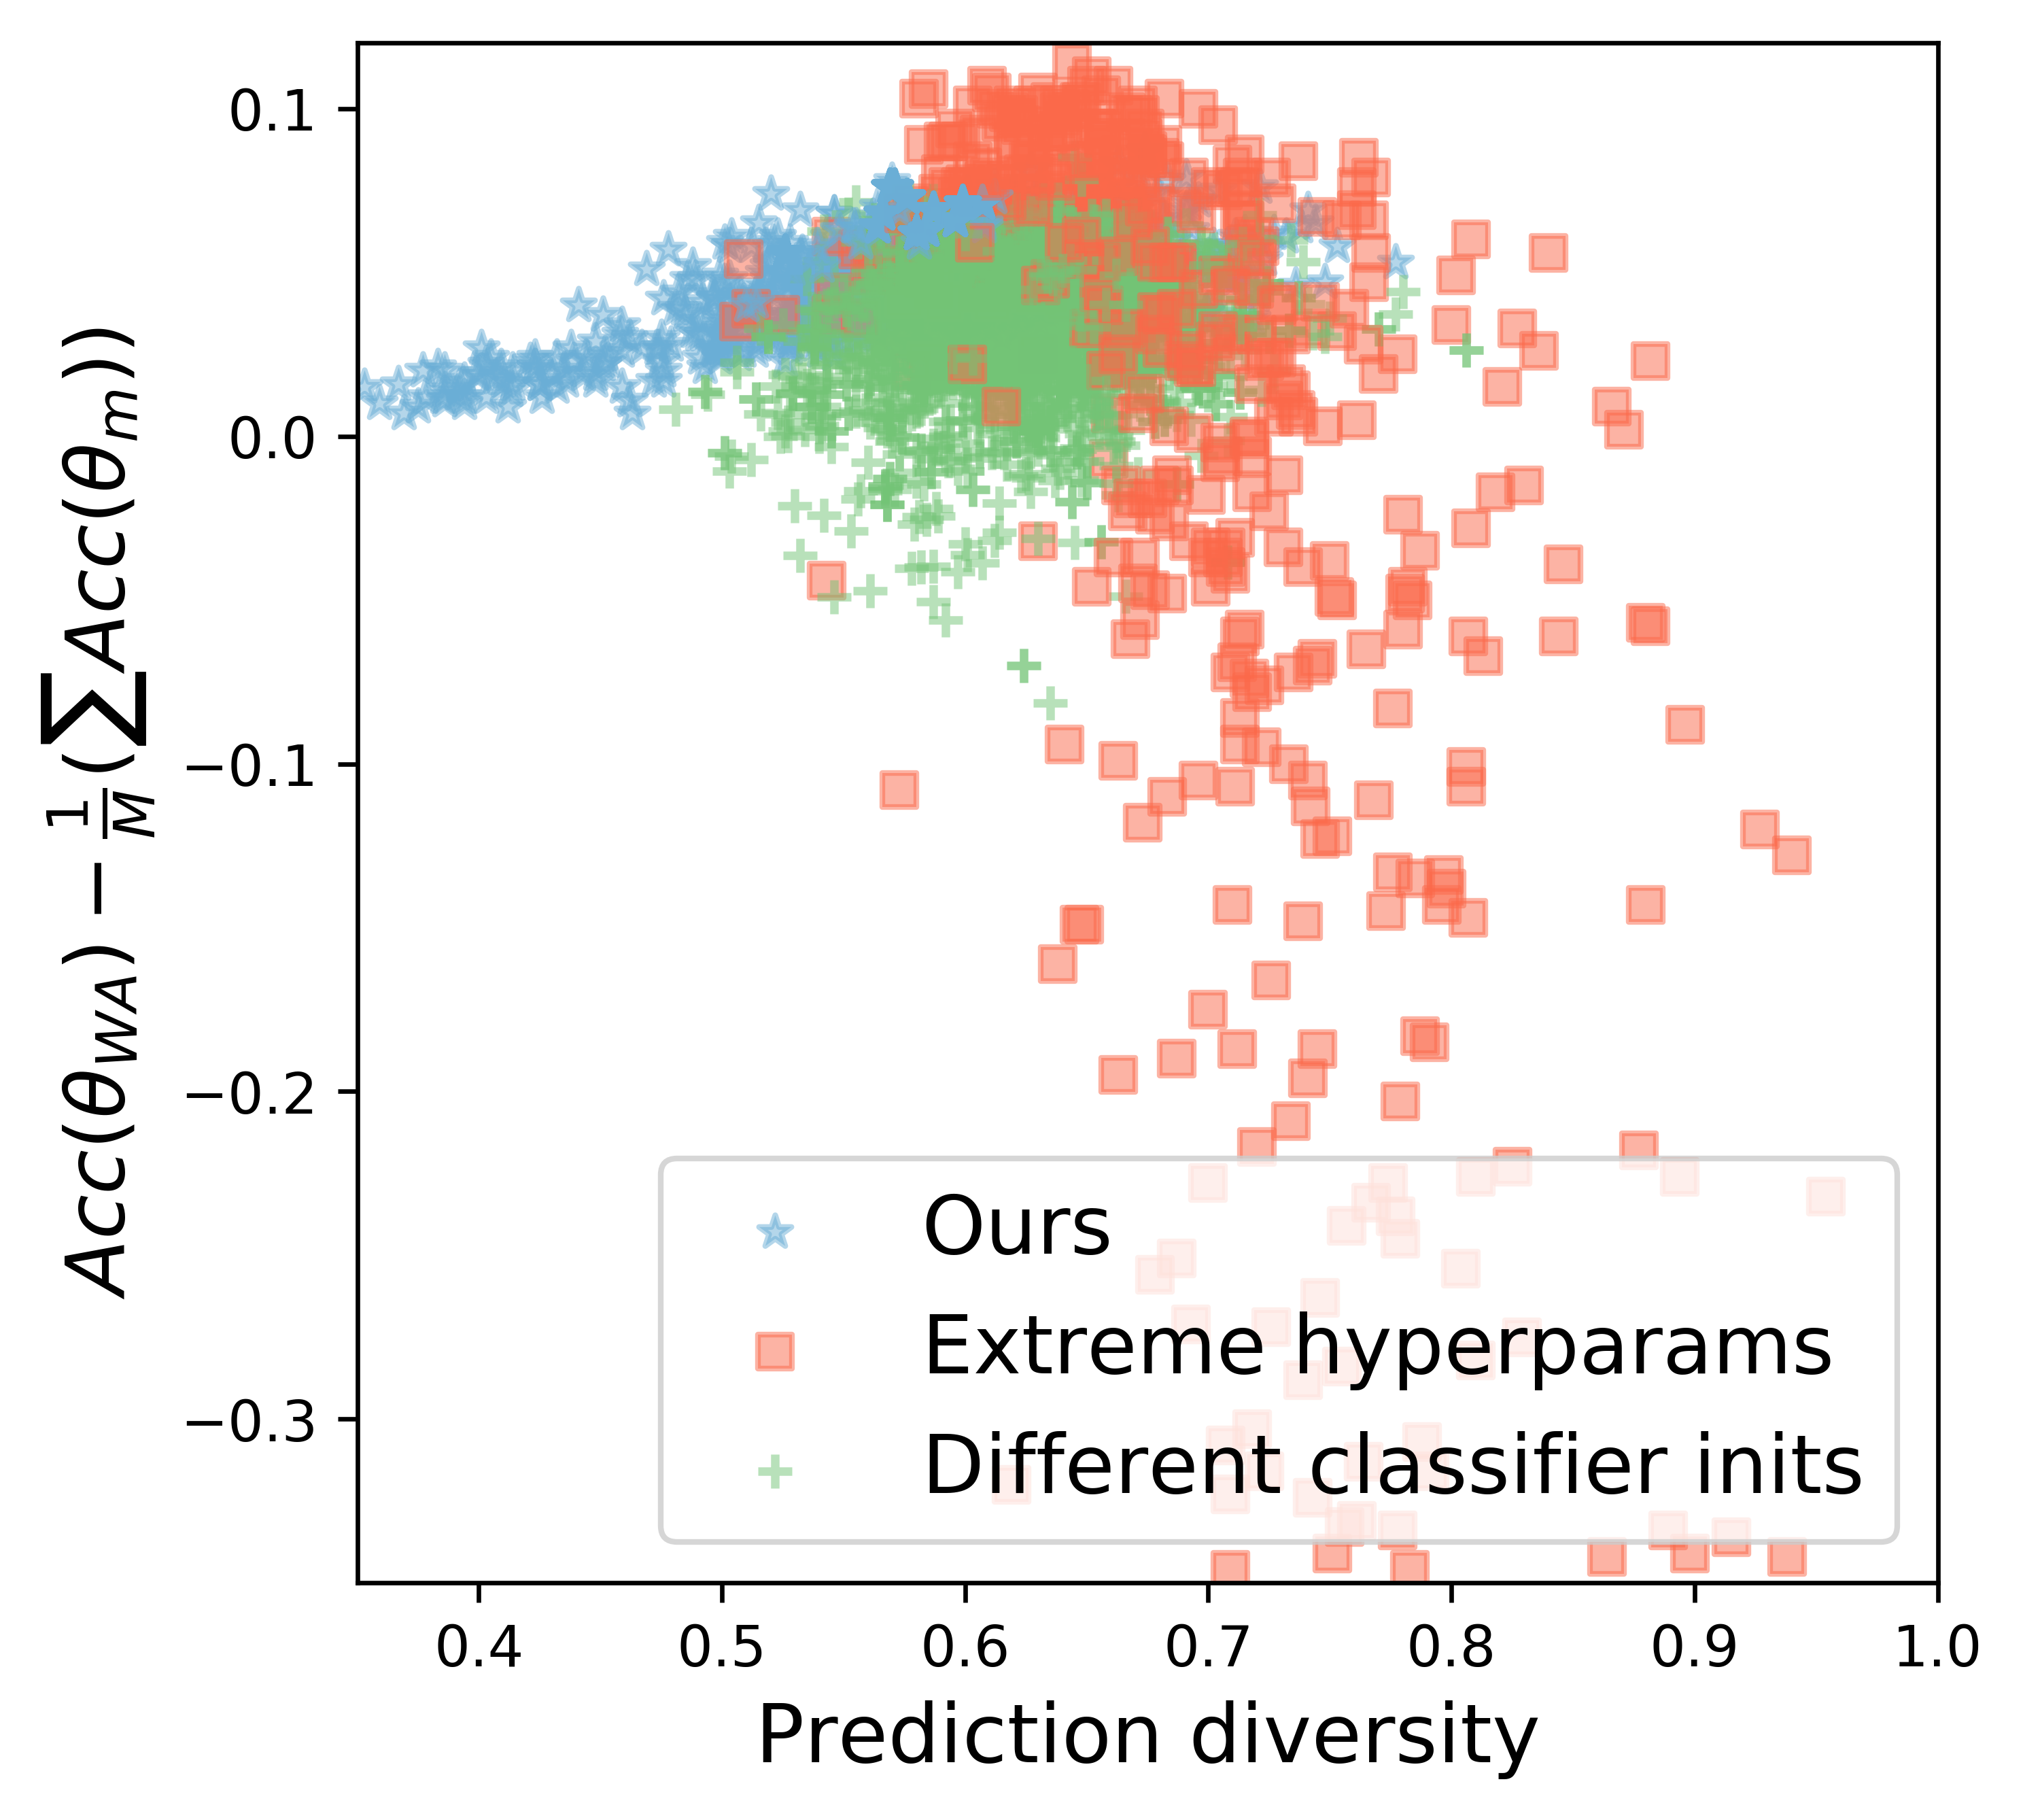
\includegraphics[width=0.9\textwidth]{pictures/files/final/home0_diffrunslargehpnosh_dr_soup-netm.png}%
%         \caption{Averaging ability.}%conditions ça ne me parait pas plus clair
%         \label{fig:home0_locality_requirement}%
%     \end{subfigure}%
%     \caption{Weights sampled from different runs are more diverse than those from a single run, and perform better after averaging, when they have close hyperparameters and shared initialization.}%
%     \label{fig:home0_dwa_vs_wa}%
%     \vspace{-1em}%
% \end{figure}%
\begin{figure}[b]
% \vspace{-0.5em}%
\begin{minipage}{.32\textwidth}%
    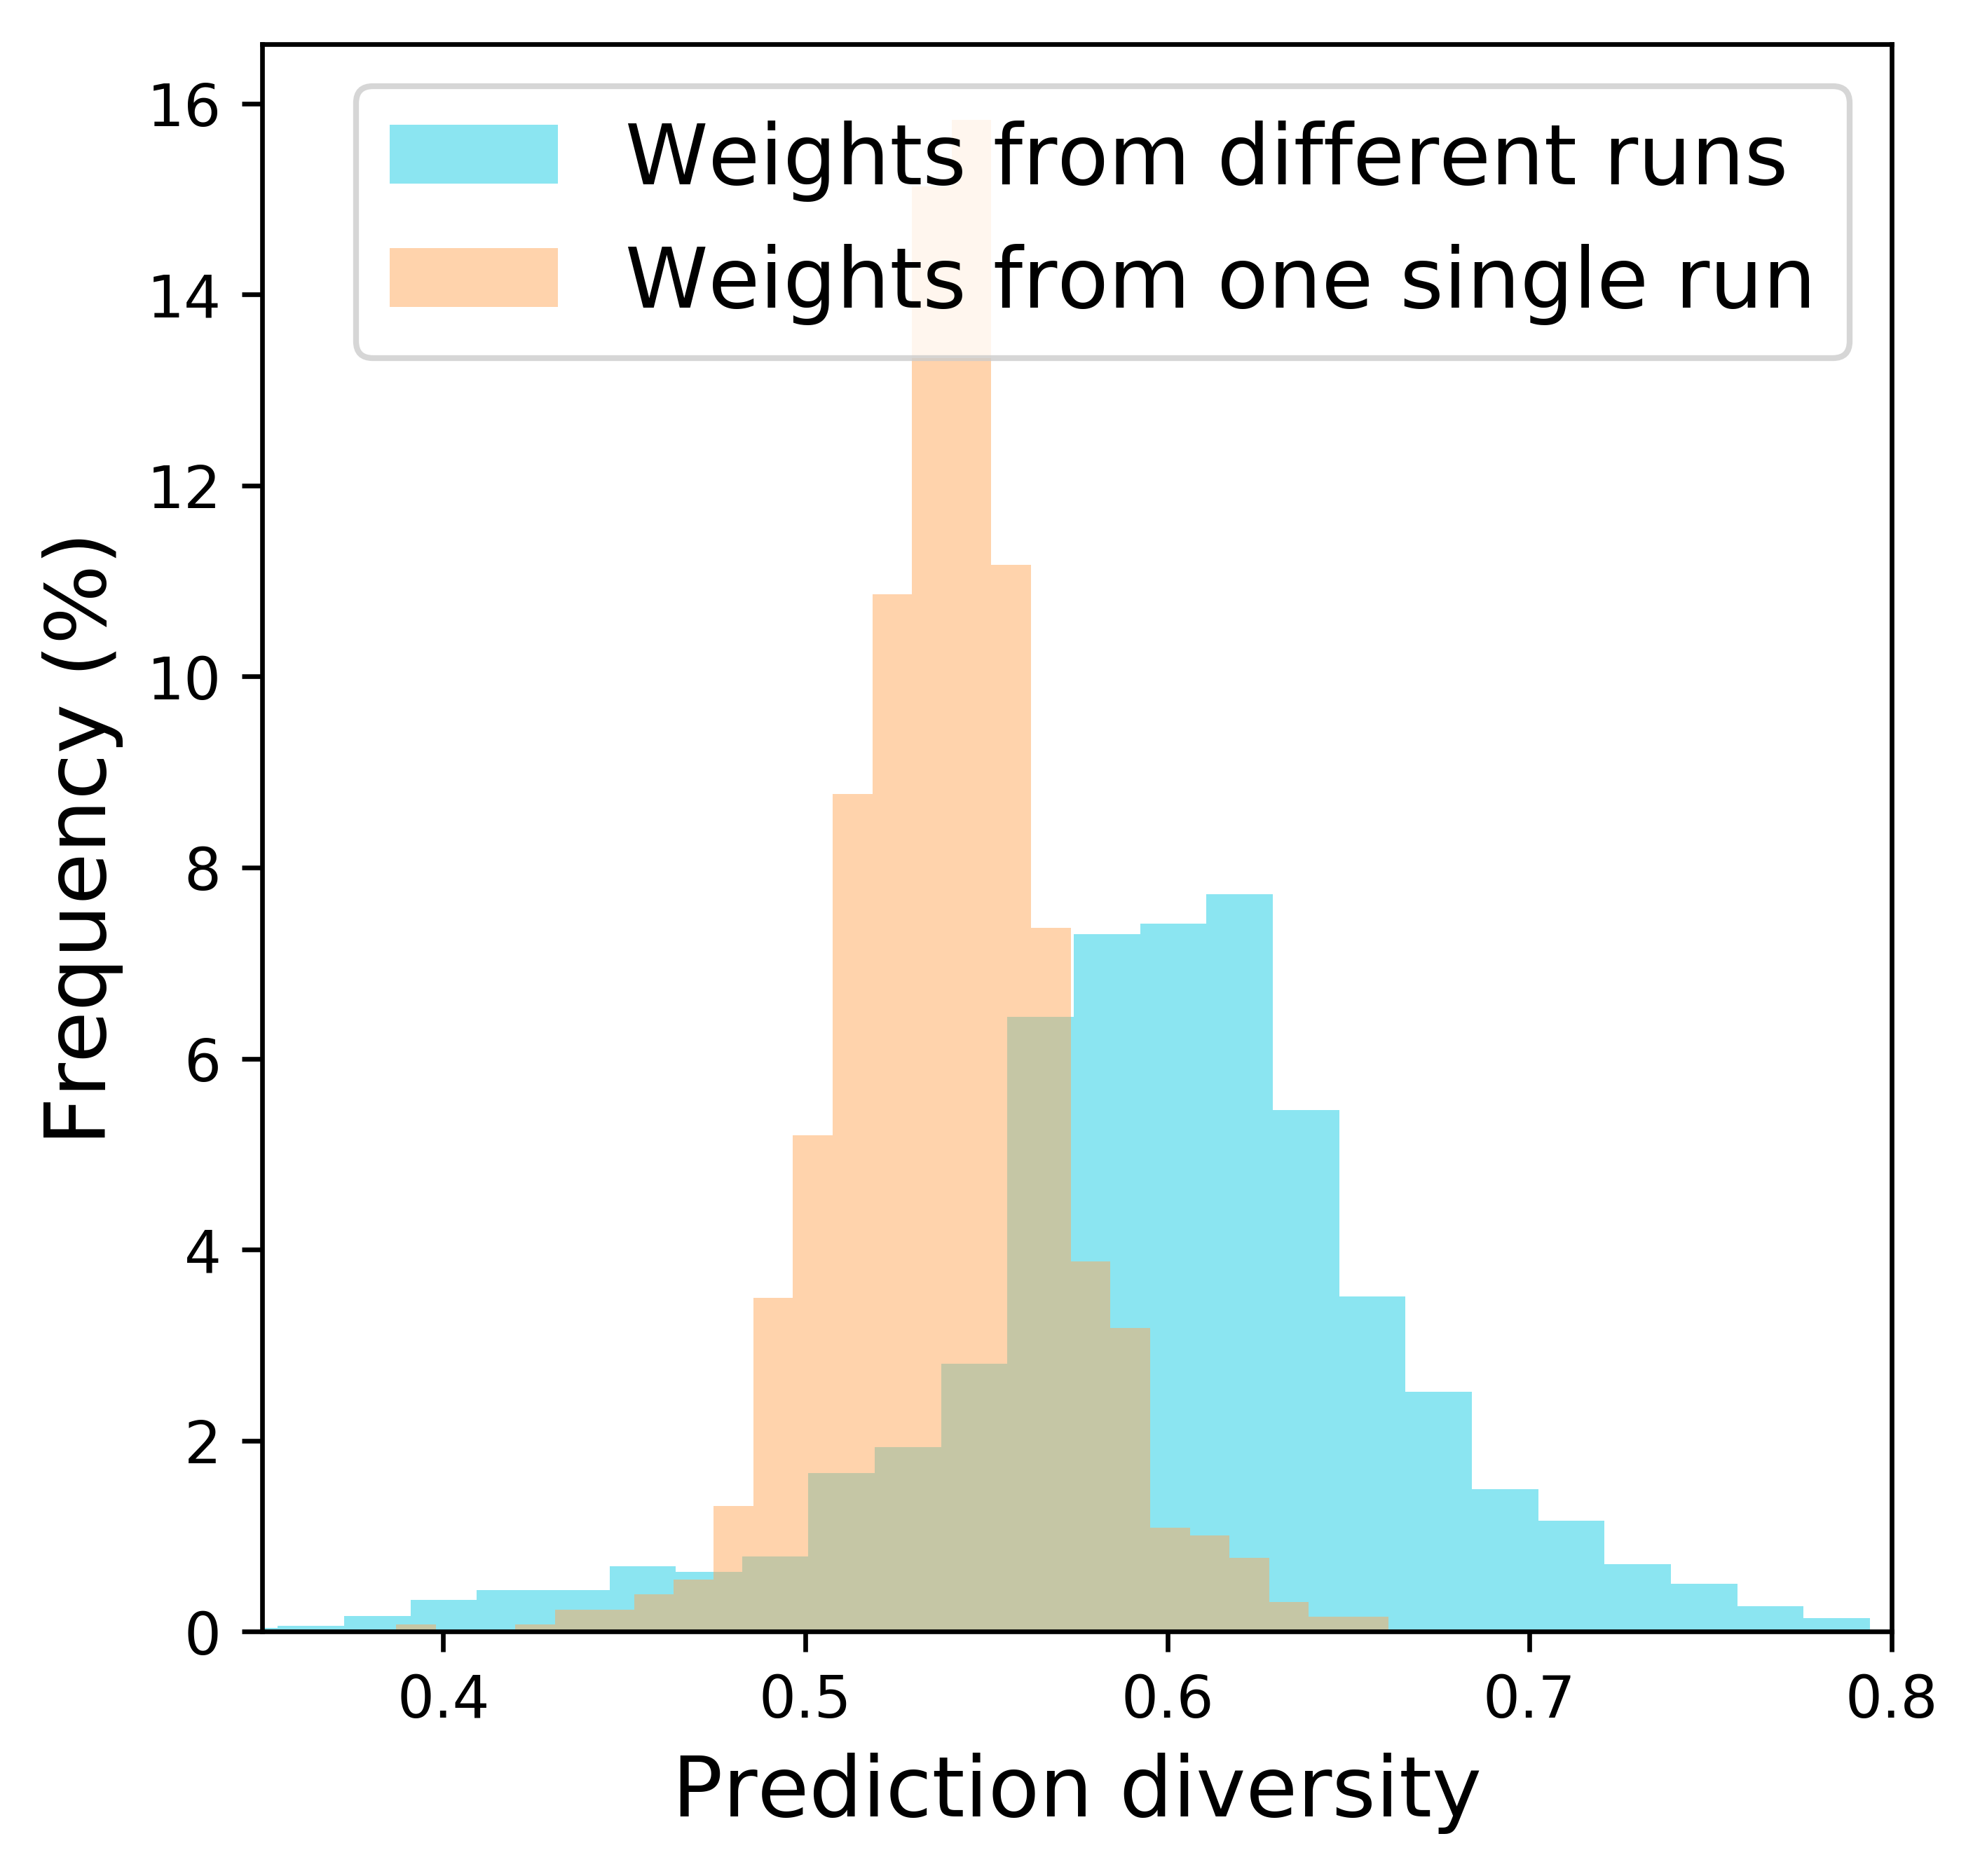
\includegraphics[width=1.0\textwidth]{pictures/files/final/home0_hist_dr.png}%
    \captionof{figure}{Frequencies of prediction diversities ($\uparrow$) \cite{aksela2003comparison} across $2$ weights obtained along a single run or from different runs.}%
    \label{fig:home0_dr_frequency}
\end{minipage}%
\hskip 1.5ex
\begin{minipage}{.32\textwidth}%
    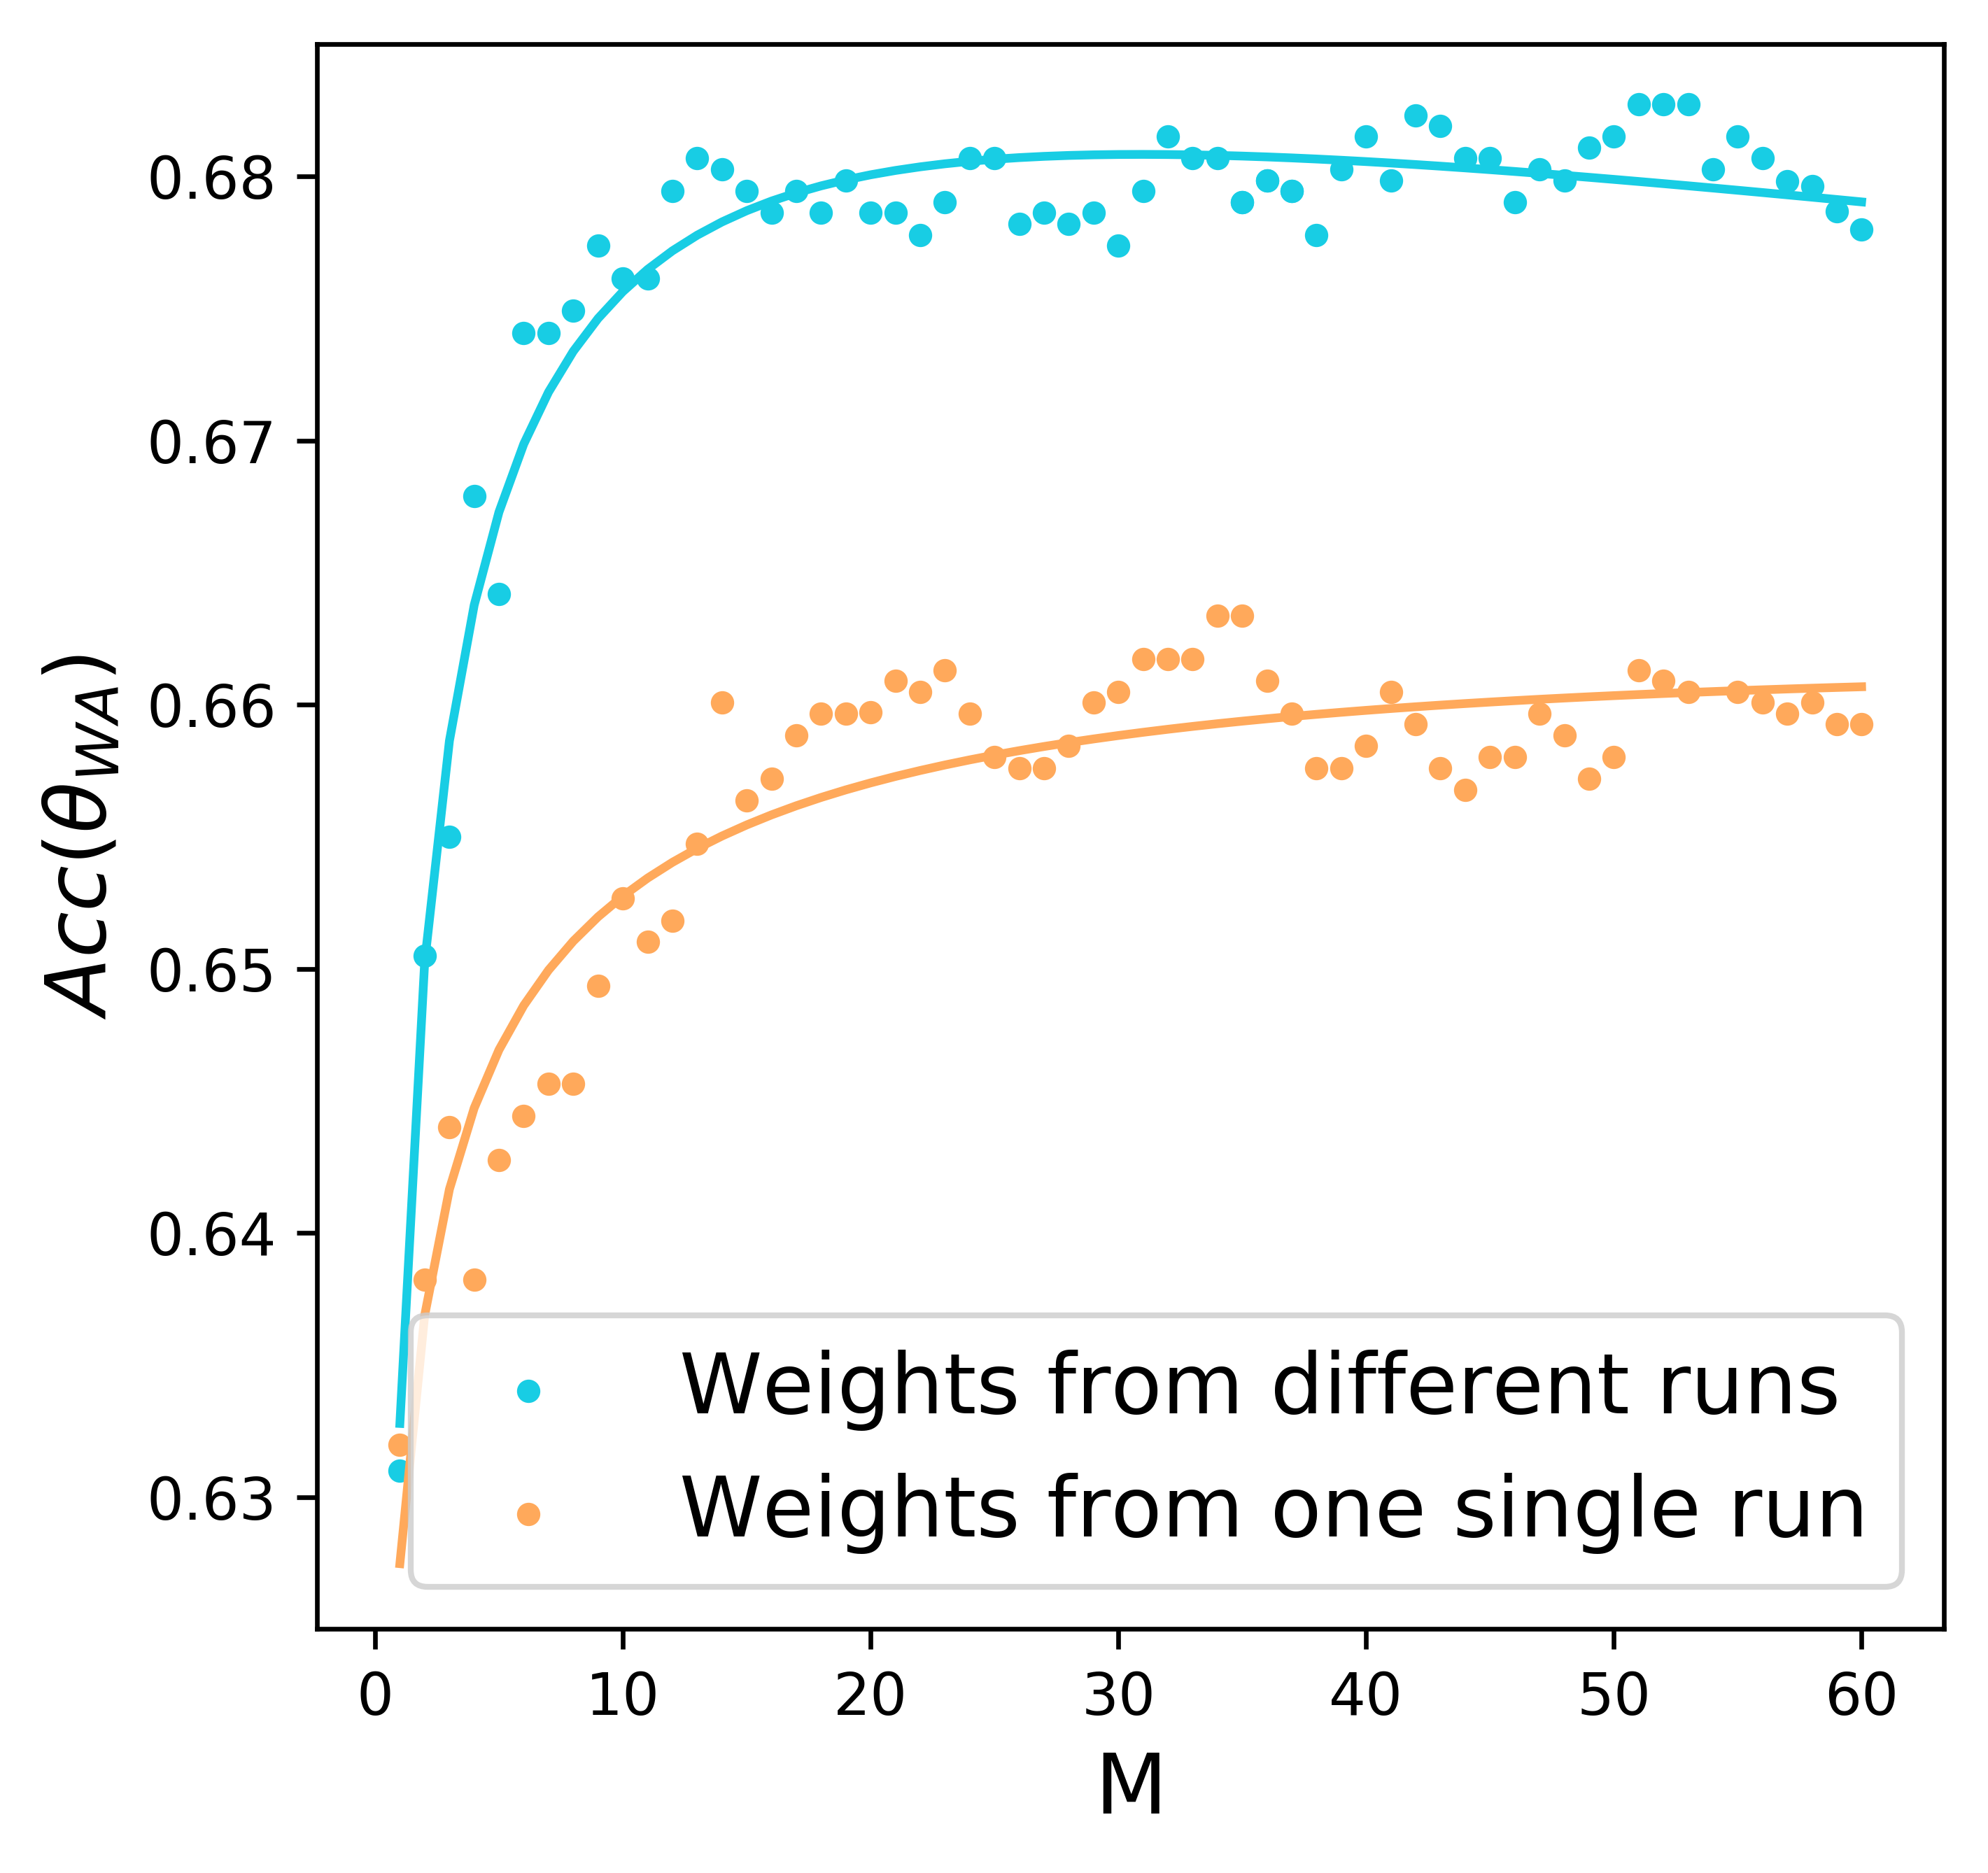
\includegraphics[width=1.0\textwidth]{pictures/files/final/home0_samediffruns_m_soup_ood.png}%
    \captionof{figure}{WA accuracy ($\uparrow$) as $M$ increases, when the $M$ weights are obtained along a single run or from different runs.}%
    \label{fig:home0_m_vs_acc}%
\end{minipage}%
\hskip 1.5ex
\begin{minipage}{.32\textwidth}%
    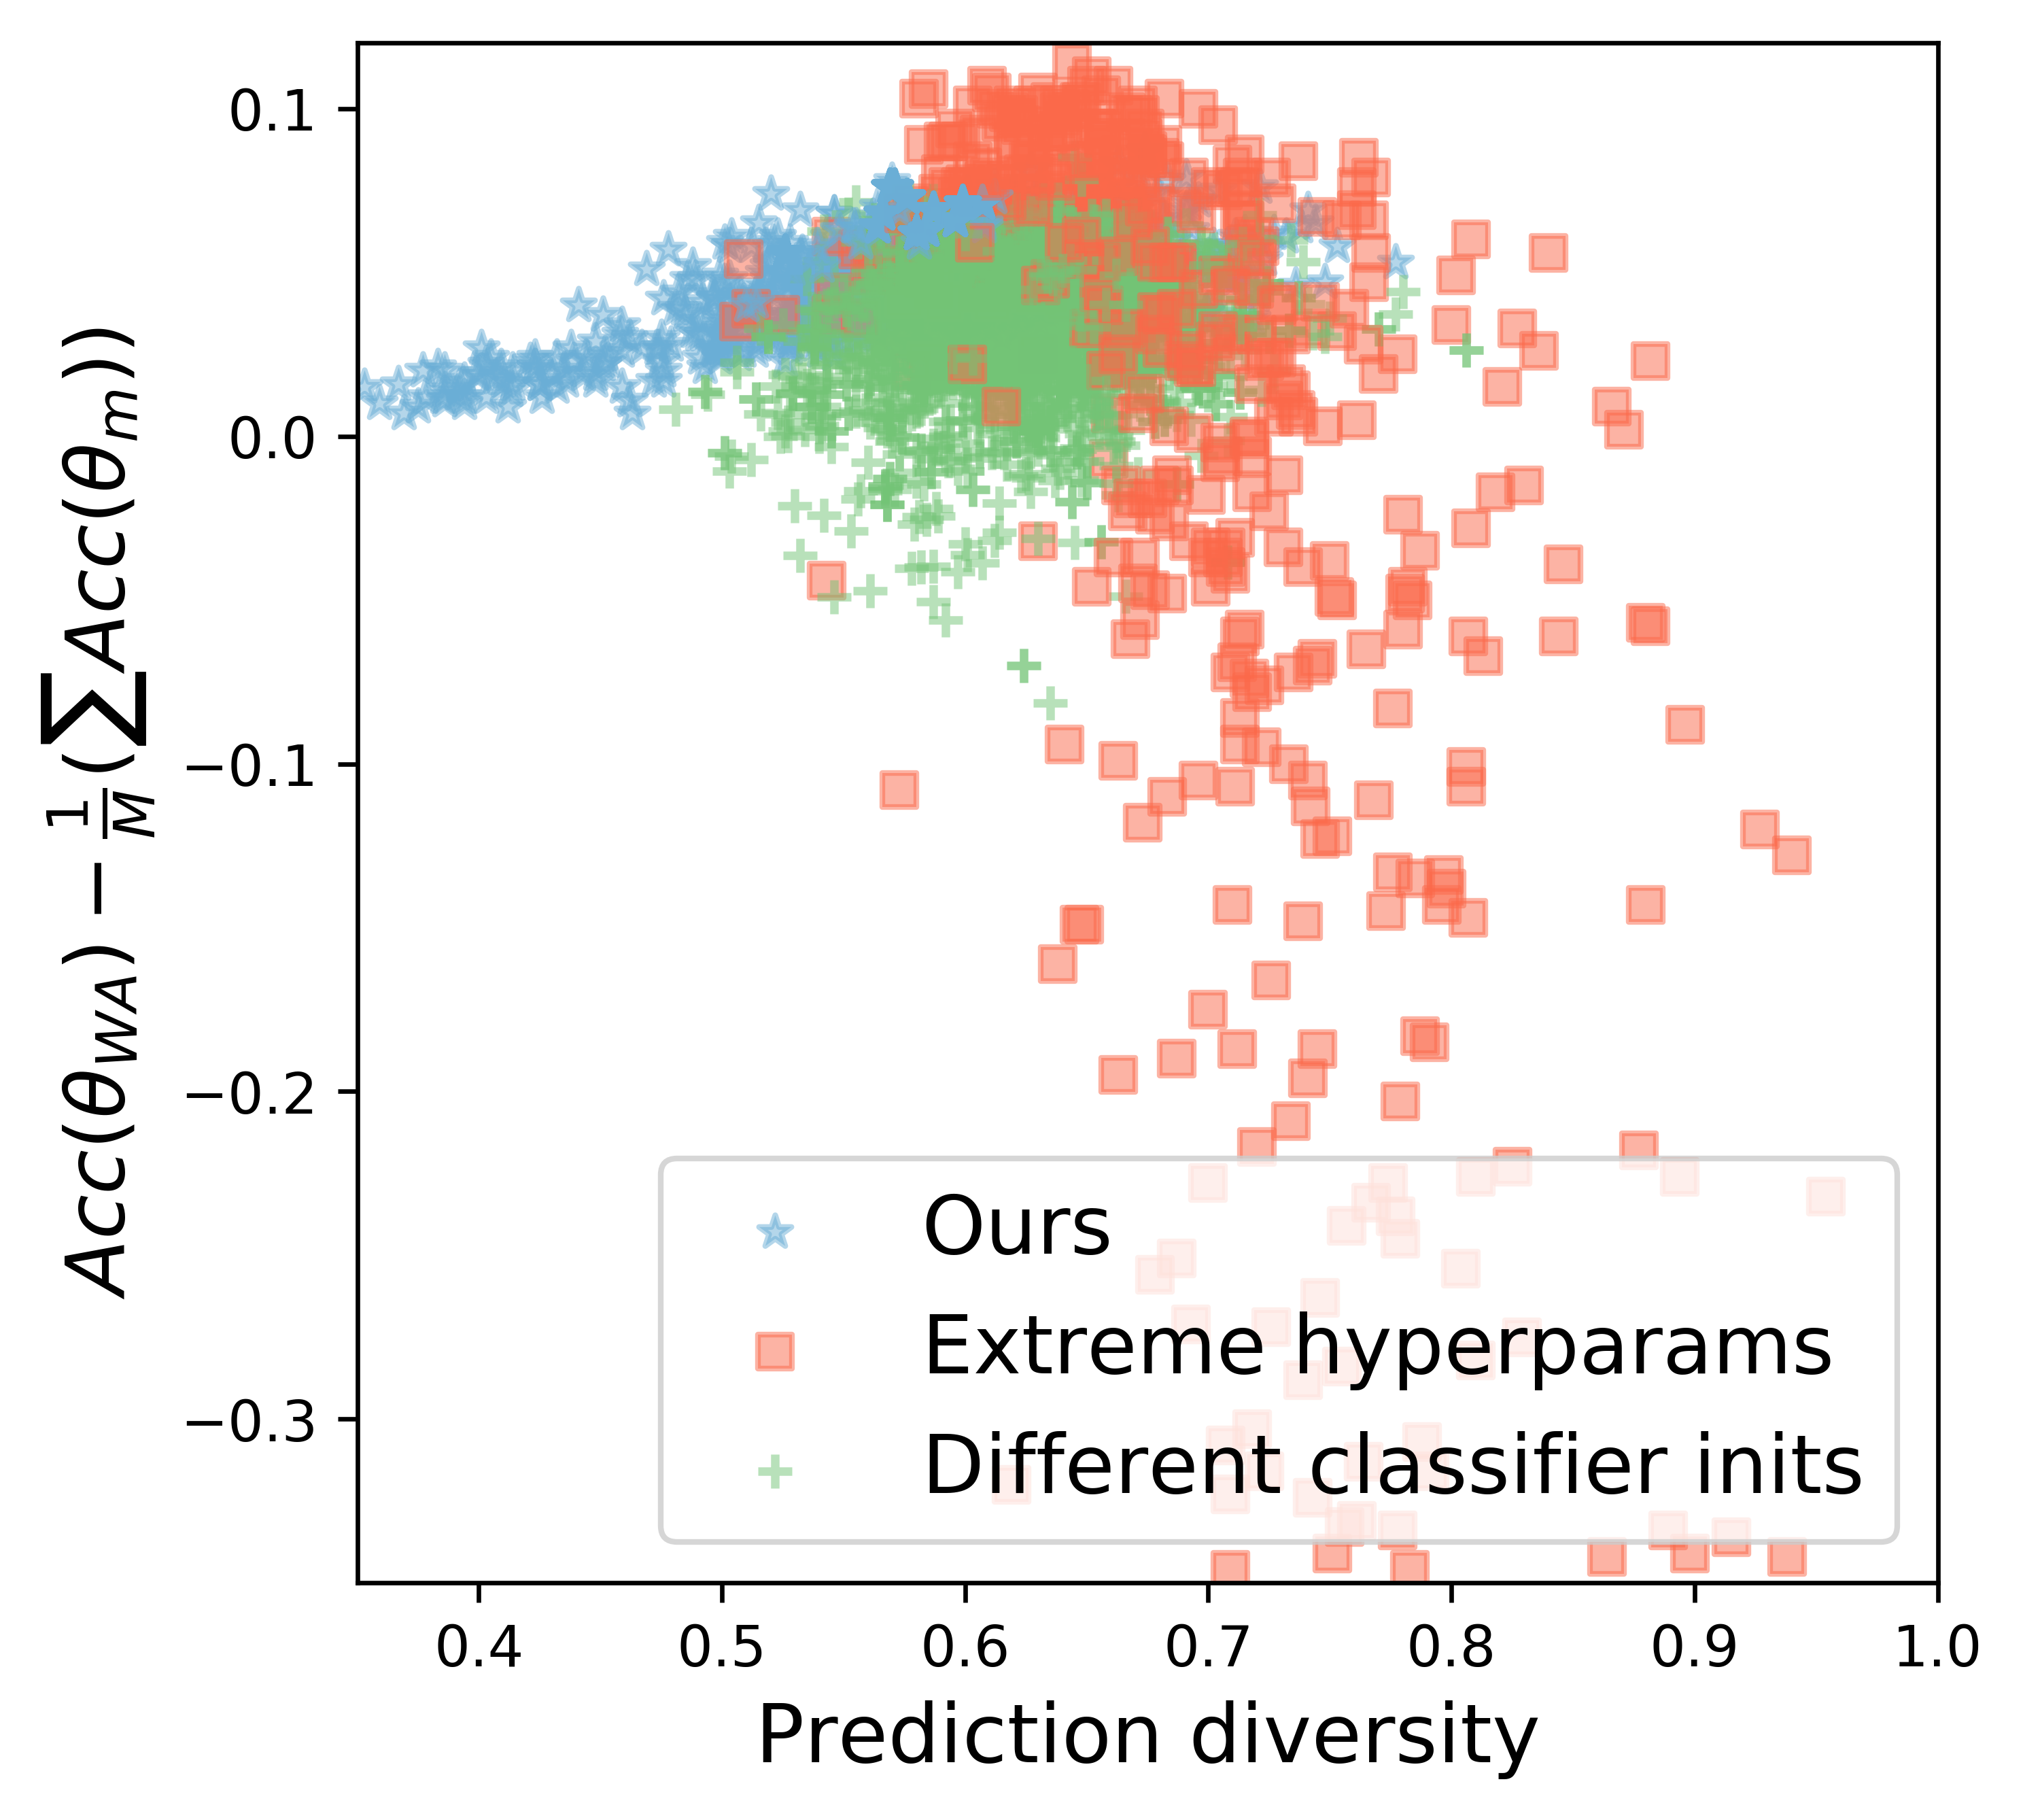
\includegraphics[width=1.0\textwidth]{pictures/files/final/home0_diffrunslargehpnosh_dr_soup-netm.png}%
    \captionof{figure}{Each dot displays the accuracy ($\uparrow$) gain of WA over its members \versus prediction diversity ($\uparrow$) for $2\leq M < 10$ models.}
    \label{fig:home0_locality_requirement}%
\end{minipage}%
\vspace{-1.em}%
\end{figure}
%